\section{Signal Extraction using the $k$-means algorithm}\label{sec:kmeans}

The two-dimensional plane described in Sec.~\ref{sec:2lss event BDT} is partitioned in several regions, depending on their different
signal or background composition, with the objective of maximizing the analysis sensitivity with the available luminosity. To do so, a recursive application of the $k$-means algorithm~\cite{MR0090073,macqueen1967} is used.

This algorithm consists of picking $k$ random points in the space: these points are taken to be the seed (``centroid'')
for clustering the data into $k$ sets. Each of the remaining data points is then associated to the closest cluster; common implementations of the algorithm are often applied preferentially to either sparse or dense data. For sparse data, and the original implementation of the algorithm, each time a point is added to a set, the centroid of that group is recomputed by taking into account the new data point. For dense data, all the points are associated to their closest cluster. In this analysis, it is assumed that the data are sufficiently dense to permit using the latter, which is computationally faster.

The $k$-means algorithm is considered very stable, and indeed preliminary tests have shown that, after fixing $k$, the algorithm converges to the same sets even when starting from many different random initial centroids.

However, the application of the algorithm to the problem of finding an effective binning to optimize the sensitivity of the analysis depends on the arbitrary choice of number of clusters.

We therefore devise a recursive version of the algorithm, which works as follows: an initial clusterization into two sets ($k=2$) is performed, and the resulting clusters are passed to the next iteration as two independent clusters. The ($k=2$)-means algorithm is applied to each of these clusters, obtaining four subclusters. This procedure can in principle be repeated until each cluster consists of a single data point: a meaningful set of clusters is instead characterized by the presence of both signal and background, in different proportions in each cluster. A stopping criterion is therefore devised, in order to stop the division of any given cluster.

The criterion of choice states that a region will not be subdivided if any of its subregions would contain less than 4~\ttH
~or less than 3~\ttbar~expected events: this ensures a reasonable signal and background population in each bin, thus protecting from hard fluctuations due to limited statistics of the samples.

This method is applied separately in the same-sign dileptonic and in the multileptonic inclusive signal regions, using two sets of simulated events from the \ttH, \ttW, and \ttbar samples.

%An orthogonal set of simulated events from the same samples is used in each signal region to ...

\begin{figure}[htb]
	\centering
        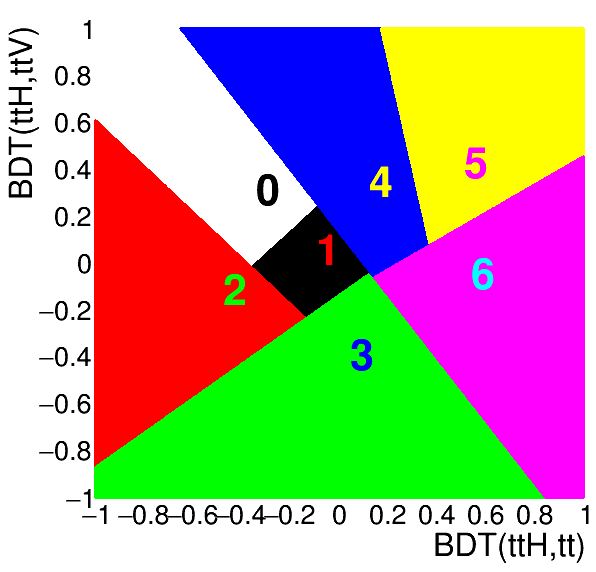
\includegraphics[width=0.35\textwidth]{plots_extraction/binning/2lss/voronoi_2l}
        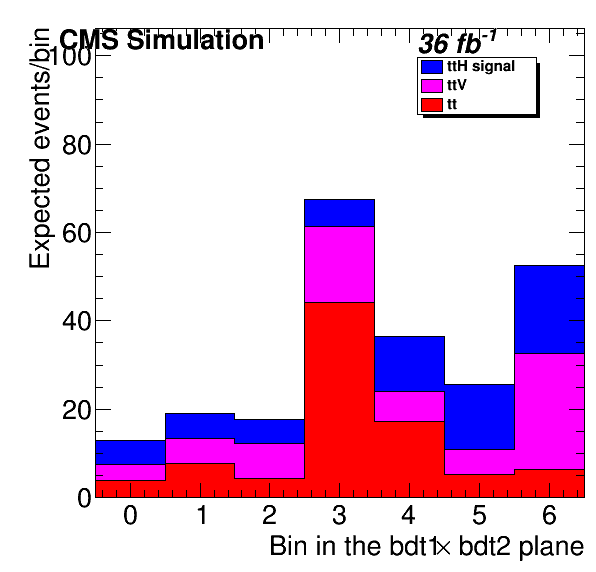
\includegraphics[width=0.35\textwidth,height=0.35\textwidth]{plots_extraction/binning/2lss/recursive_2l}
        \caption{The location of the different bins in the two-dimensional plane (left), as well as the number of expected events in each bin (right) in the two same sign leptons channel, estimated from MC.}
	\label{fig:2l_2dbinning}
\end{figure}


\begin{figure}[htb]
	\centering
        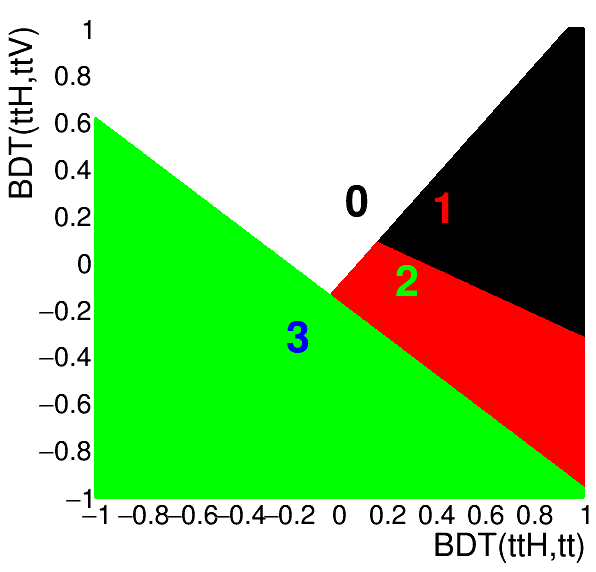
\includegraphics[width=0.35\textwidth]{plots_extraction/binning/3l/voronoi_3l}
        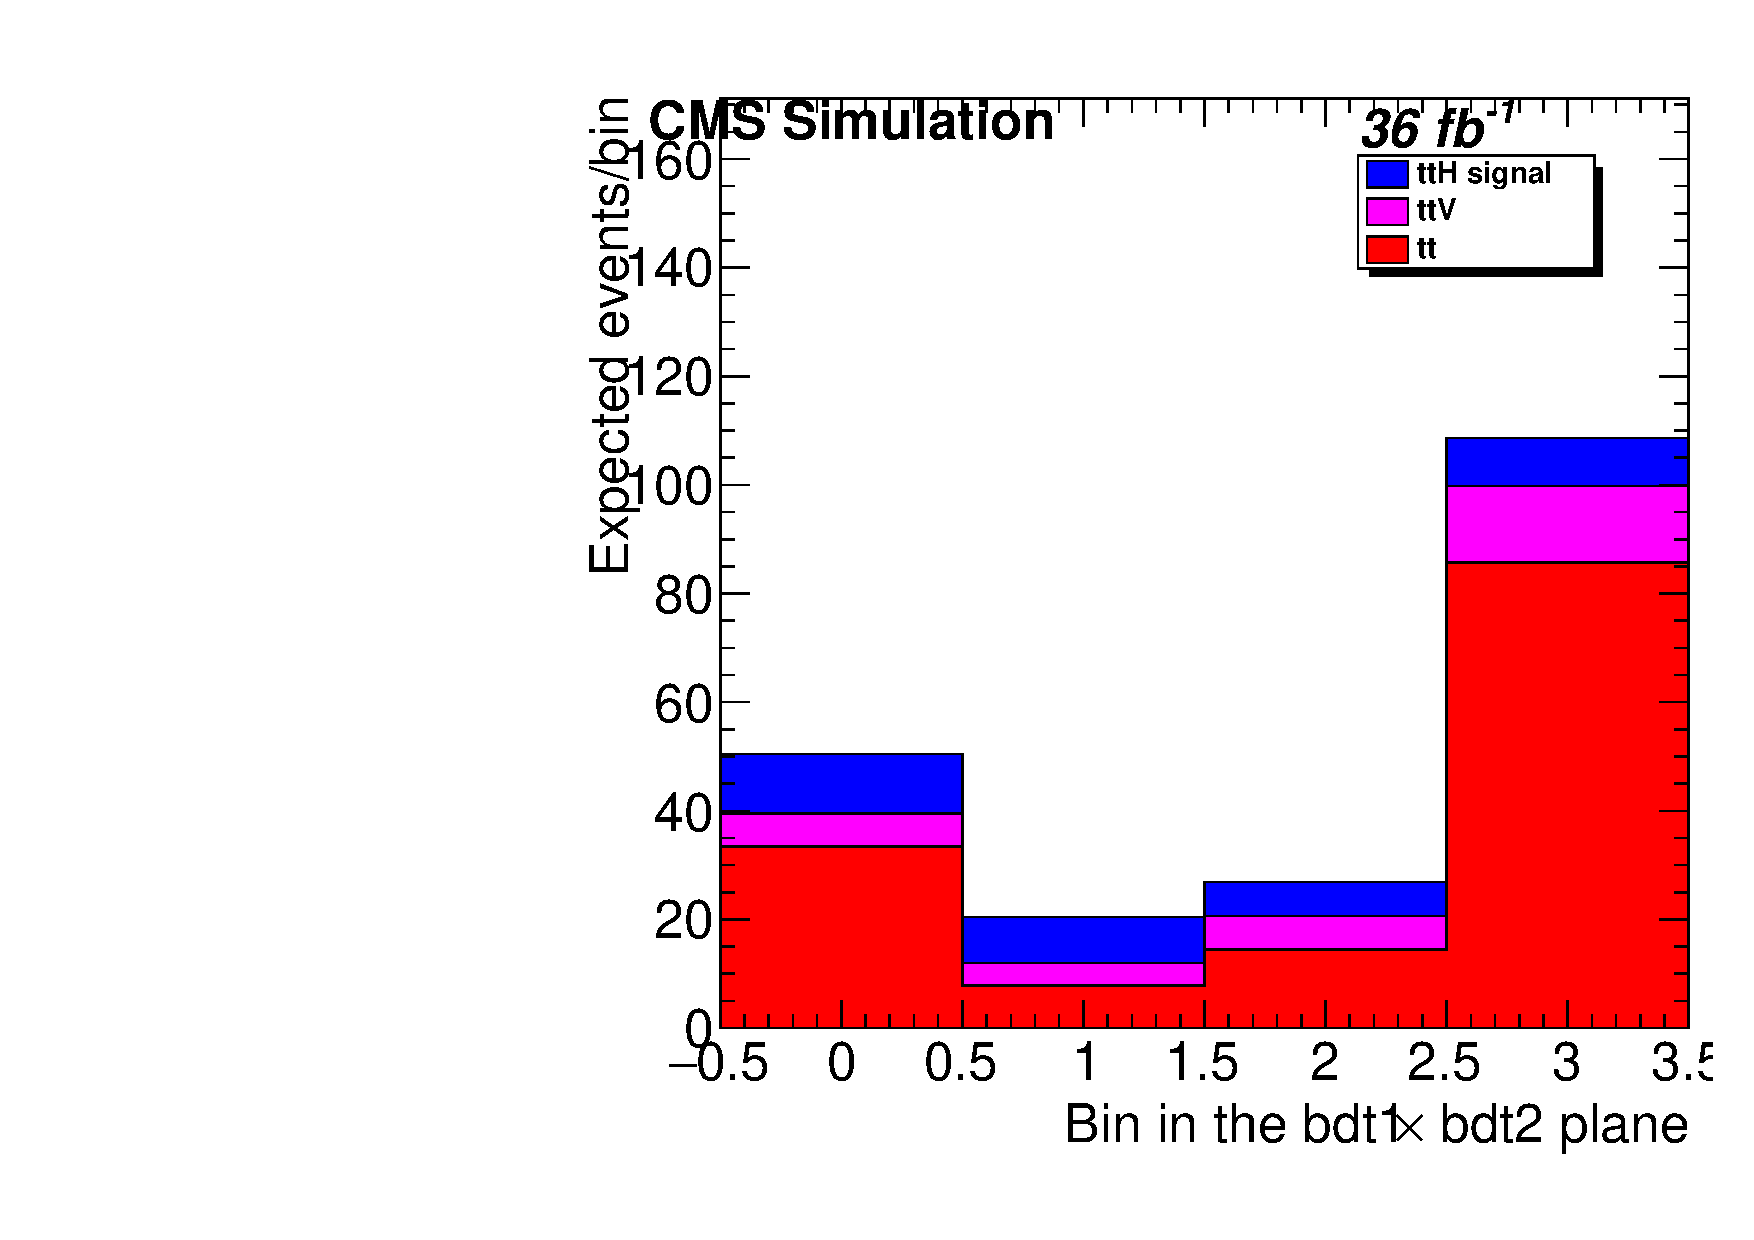
\includegraphics[width=0.35\textwidth,height=0.35\textwidth]{plots_extraction/binning/3l/recursive_3l}
        \caption{The location of the different bins in the two-dimensional plane (left), as well as the number of expected events in each bin (right) in the three leptons channel, estimated from MC.}
	\label{fig:3l_2dbinning}
\end{figure}

Figures~\ref{fig:3l_2dbinning} and~\ref{fig:2l_2dbinning} show -- for the two same sign leptons and multileptonic inclusive regions, respectively -- the location of the different bins in the two-dimensional plane (left), as well as the number of expected events in each bin (right).
%after reordering the bins by increasing signal to background ratio (right).

Similar results are obtained with an alternative method, in which each
subdivision is obtained by applying cuts of the type $a \textrm{MVA}_{ttW} + b < \textrm{MVA}_{t\bar{t}}$,
where $a$ and $b$ are parameters chosen to optimize some figure-of-merit (FOM). The FOM chosen
is $\mathcal{P}(s_1 + b_1\ \| \ b_1)  \mathcal{P}(s_2 + b_2\ \| \ b_2)$, where $\mathcal{P}(x\ \| \ \mu)$
represents the Poisson probability and $s_{1(2)}$, $b_{1(2)}$ are the number of signal and background events in each subdivision.

%Figures~\ref{} show the location of ...
